\documentclass[11pt,a4paper]{article}
\usepackage{RaccaStyle-en}
\usepackage{RSMatematica}
\usepackage{RSProgrammazione}
\usepackage{cprotect}

\begin{document}
\thispagestyle{empty}

\rmfamily
\begin{center}
\ \\
\vspace{2cm}

\LARGE{\textcolor[rgb]{1,0,0}{REPORT FOR THE PROJECT\\ for the exam of\\BIG DATA SCIENCE AND MACHINE LEARNING}\\}
\hrulefill \\
\huge{\textcolor[rgb]{1,0,0}{\ \\Computation of Napier's constant}\\}
\hrulefill \\
\vspace{1.5cm}

\Large{Academic Year 2021/2022
\\ \ \\
Professors: GABRIELE GAETANO FRONZÉ\\
FEDERICA LEGGER\hspace{4.2cm} \\
\hspace{-1cm}SARA VALLERO\hspace{15.2cm} \\
\ \\ \ \\ 
Candidate: RACCA ELEONORA}

\vspace{5cm}
\begin{figure}[h]
\centering
	\includegraphics[width=0.3\textwidth]{../Images/ScuolaDottoratoUnito.pdf} 
	\hspace{5mm} 
	
\includegraphics[width=0.3\textwidth]{../Images/ScuolaDottoratoFisica.pdf}
\end{figure}

\end{center}

\newpage
\section{Introduction}
\par Sequential programming can be very time consuming, even with the fastest CPUs available.
For this and for many other reasons in the last two decades it is becoming more and more common the parallel computing.
This way of programming exploits many CPUs simultaneously, reducing the time needed for repetitive computation tasks.
\par The aim of this project is to compare the performances of different implementations of parallel computation while calculating the Napier's constant.
The computing model used to develop the algorithms in this project is \textsc{OpenMP}.

\subsection{Napier's constant}
\par The Napier's constant $\esp$ is a mathematical constant used for many applications across all sciences.
It is included in the Euler's identity with the other four most important mathematical constants:
$$\esp ^{i \pi} + 1 = 0$$
$\esp$ is an irrational and a transcendental number, and its first 50 decimal places are:
$$2.71828182845904523536028747135266249775724709369995$$
Its name is taken after John Napier, a Scottish mathematician, physicist and astronomer. 
Sometimes it is also called Euler's number, after the Swiss mathematician Leonhard Euler, even though it was discovered  by the Swiss mathematician Jacob Bernoulli.
\par $\esp$ can be defined in many different ways, for example it can be defined as the base of the natural logarithm or the limit
$$\esp = \lim _{n \to 0} {\left( 1 + \frac{1}{n} \right)}^n$$
A convenient way to compute it while taking advantage of the parallel computation is its infinite series:
\begin{equation}
\label{eq:Napier}
\esp = \sum_{n = 0} ^{\infty} \frac{1}{n!}
\end{equation}
\par In this project the Napier's number $\esp$ is calculated with \equaname~1.
As it is impossible to do the calculation until $\infty$, the maximum number considered for $n$ is $100000$.

\subsection{The Code}
\par The code used to compute the calculation can be found in the \textsc{GitHub} repository:
\begin{verbatim}
https://github.com/eleoracca/MLCourse-2122
\end{verbatim}
in the subfolder \verb+OpenMP-Exam+.
\par After cloning the \textsc{GitHub} repository to a local folder, it is possible to compile and execute the code locally without adjustments.
To compile the code, the following command is needed:
\begin{verbatim}
g++ -o nepero -fopenmp Nepero.c
\end{verbatim}
To execute the code, it is sufficient to launch the newly created executable, which will perform all the functions needed for the comparison.
\par The code is made of seven functions:
\begin{itemize}
	\item \verb+main+: which defines the maximum value of $n$ and calls for the functions that perform each parallel computation;
	\item \verb+factorial+: which is called by all the functions performing the parallel computations and calculates the factorial of a given number $n$;
	\item \verb+range+: which performs the parallel computation assigning a user-defined portion of the \verb+for+ loop to each thread;
	\item \verb+forsimple+: which performs the parallel computation using the \verb+for+ loop refactored by \textsc{OpenMP};
	\item \verb+forcritical+: which performs the parallel computation combining the \verb+for+ loop with the \verb+critical+ statement of \textsc{OpenMP} to avoid the race conditions;
	\item \verb+foratomic+: which performs the parallel computation combining the \verb+for+ loop with the \verb+atomic+ statement of \textsc{OpenMP} to avoid the race conditions;
	\item \verb+forreduction+: which performs the parallel computation combining the \verb+for+ loop with the \verb+reduction+ statement of \textsc{OpenMP} to avoid the race conditions;
\end{itemize}
\par The structure of the functions, which perform the parallel computations, is always the same.\\
At the beginning the global variables are defined, which are: the file on which export the results; the variable \verb+e+ with the sum at each step of the loop; the time variables, to compute the elapsed time.
In the functions \verb+range+ and \verb+forsimple+, the variable \verb+e+ is defined as a vector and it is also necessary to have an additional variable \verb+thread_id+ which takes into account which thread is working.\\
Following the declarations, is the \verb+for+ loop, which loops on the number of threads from $1$ to the maximum available on the specific computer used.
In this \verb+for+ loop, a nested \verb+for+ loop computes the parallelised calculation of the Napier's constant and the time variables record the passing of time.
At the end of the computation, the elapsed time and the value of $\esp$ are printed.\\
At the end of the \verb+for+ loop on the number of available threads, the execution of the function stops and the \verb+main+ function calls the next computation function.

\section{Parallel execution in for loops}
\par To parallelize the algorithms with \textsc{OpenMP}, the \verb+pragma+ directives are needed.
In particular it is necessary to activate the environment
\begin{verbatim}
#pragma omp parallel
\end{verbatim}
Inside this scope, there are two main ways to parallelize the \verb+for+ loop in \textsc{OpenMP}:
\begin{enumerate}
	\item code the \verb+for+ loop in the usual way, but defining appropriate ranges for each thread;
	\item use the \verb+pragma+ directive
		\begin{verbatim}
		#pragma omp for
		\end{verbatim}	 
\end{enumerate}
\par In the project, both the possibilities were developed in order to compare the performances of the two.
The comparison was done using the resources available in the yoga platform of \textsc{INFN}, with 64 threads.\\
The code uses two different functions:
\begin{enumerate}
	\item \verb+range+, which implements the computation of the  \verb+for+ loops using user-defined ranges;
	\item \verb+forsimple+, which implements the \verb+pragma+ directives.
\end{enumerate}
\par In \figurename~1 is represented the elapsed time as a function of the number of threads used for the computation.
In violet is represented the elapsed time using the function \verb+range+, while in green is the elapsed time of the \verb+forsimple+ function.\\
As can be seen, the \verb+range+ function is slightly better in terms of time performances with respect to the \verb+forsimple+ function.
This is a bit strange, because the \verb+pragma+ directives are usually more optimised and thus using them improves the elapsed time.\\
For both the functions, it can be seen that the time is greatly reduced when using more threads, but this behaviour saturated at about $1$ second.
This is due to the fact that parts of the codes are sequential.
Furthermore, over 45 threads, great variations can be observed in the elapsed time: this can be due to the fluctuations of the usage of the threads.

\begin{figure}[h!]
	\centering
	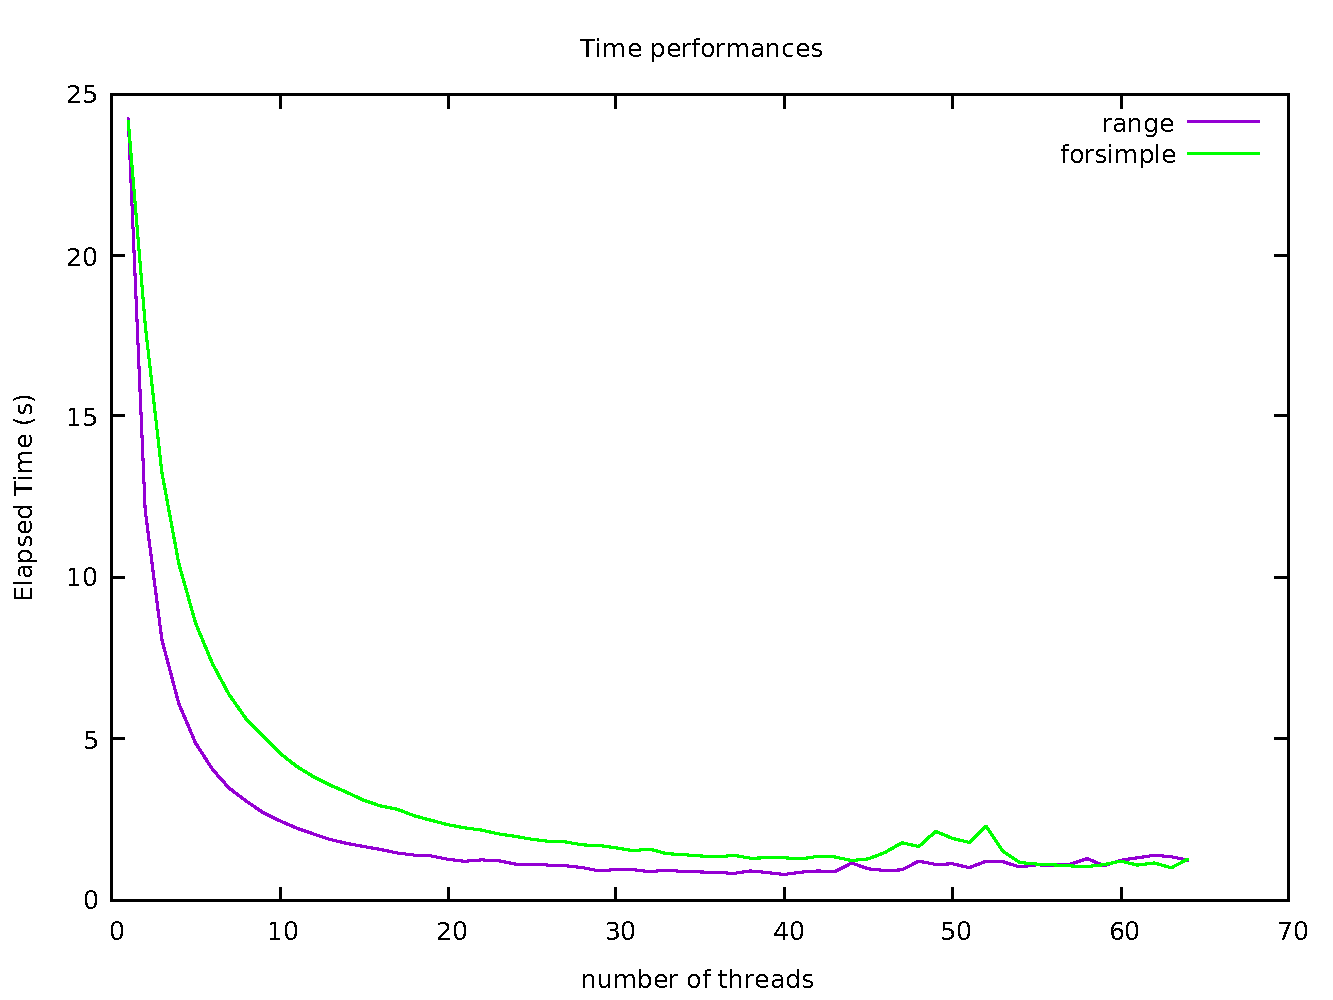
\includegraphics[width=0.75\textwidth]{../Images/Performance.pdf}
	\label{fig:loop}
	\cprotect\caption{Elapsed time as a function of the number of threads for the functions \verb+range+ (violet, no specific \verb+pragma+ directive) and \verb+forsimple+ (green, with \verb+pragma for+ directive).}
\end{figure}

\section{Avoiding race conditions}
\par In the  \verb+range+ and \verb+forsimple+ the variable \verb+e+, with the sum at each step of the \verb+for+ loop, is defined as a vector, as long as the number of threads.
At the end of the computation, the elements of the vector are summed to evaluate the number of $\esp$.
This in principle leads to longer elapsed times, as the sequential part of the code increases.
\par A way to improve this situation is to use the same variable for all the loops of the different threads.
In this case race conditions may occur: these are due to the fact that many threads try to access the same variable at the same time and the result of the computation may be overwritten in the wrong way.\\
To avoid this problem, there are three possible \verb+pragma+ directives:
\begin{enumerate}
	\item \verb+critical+, which allows one thread access the memory space of the variable and  makes the others wait for the first to finish;
	\item \verb+atomic+, which protects a specific operation for that variable, for example only one thread can update the variable, but all of them can read its value at the same time;
	\item \verb+for reduction (e:sum)+, which is a directive of the \verb+for+ loop that creates private copies of the variables for all the threads and at the end performs the desired operation.
\end{enumerate}
\par In \figurename~2 is again represented the elapsed time as a function of the number of threads used for the computation.
In blue is represented the elapsed time using the function \verb+forreduction+, which implements the \verb+for reduction (e:sum)+ directive, while in green is the elapsed time of the \verb+forsimple+ function, in which the variable \verb+e+ is defined as a vector.\\
As can be seen and can be expected, the performances are very similar.
In fact in both cases the threads have their own variable in which the partial computation is stored and at the end all of them are summed.

\begin{figure}[h!]
	\centering
	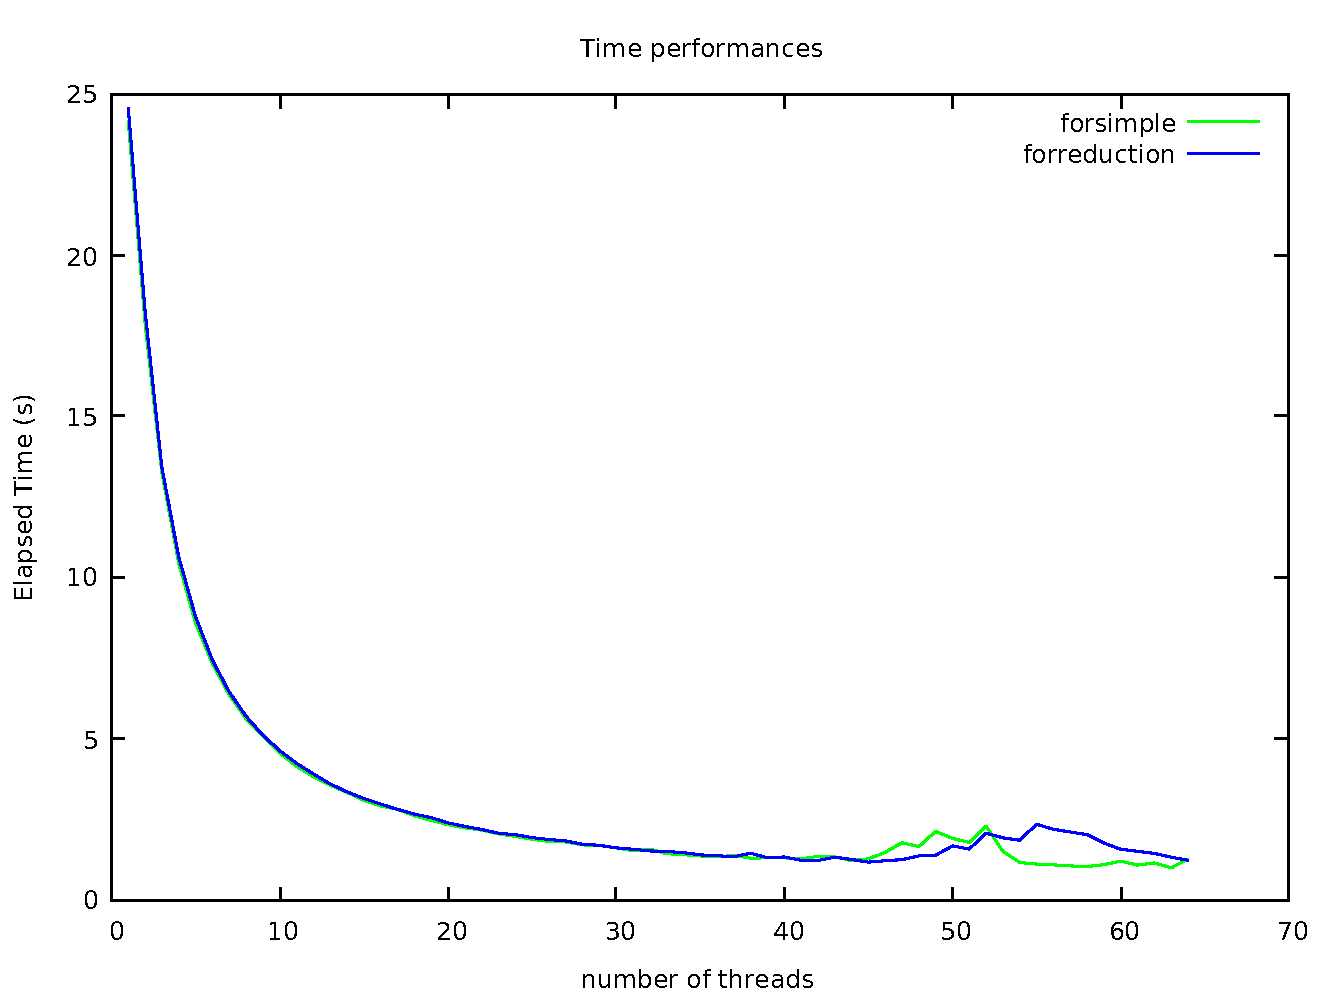
\includegraphics[width=0.75\textwidth]{../Images/Performance3.pdf}
	\label{fig:compare}
	\cprotect\caption{Elapsed time as a function of the number of threads for the functions \verb+forsimple+ (green, with \verb+pragma for+ directive) and \verb+forreduction+ (blue, with \verb+pragma for reduction+ directive).}
\end{figure}

\par In \figurename~3 is, for the third time, represented the elapsed time as a function of the number of threads used for the computation.
In this case the curves represented are the elapsed times measured by using the functions \verb+forcritical+ in violet, \verb+foratomic+ in green and \verb+forreduction+ in blue.
They implement the directives \verb+critical+, \verb+atomic+ and \verb+for reduction (e:sum)+ respectively.\\
The time performances are very similar, even though in principle the \verb+critical+ and \verb+atomic+ should be slightly slower as only one thread can access the variable dedicated for the sum.
In this case it can also be seen that when having a lot of threads, there are fluctuation in the elapsed time, but it seems that in this case the \verb+forcritical+ and the \verb+foratomic+ functions are slightly more stable.

\begin{figure}[h!]
	\centering
	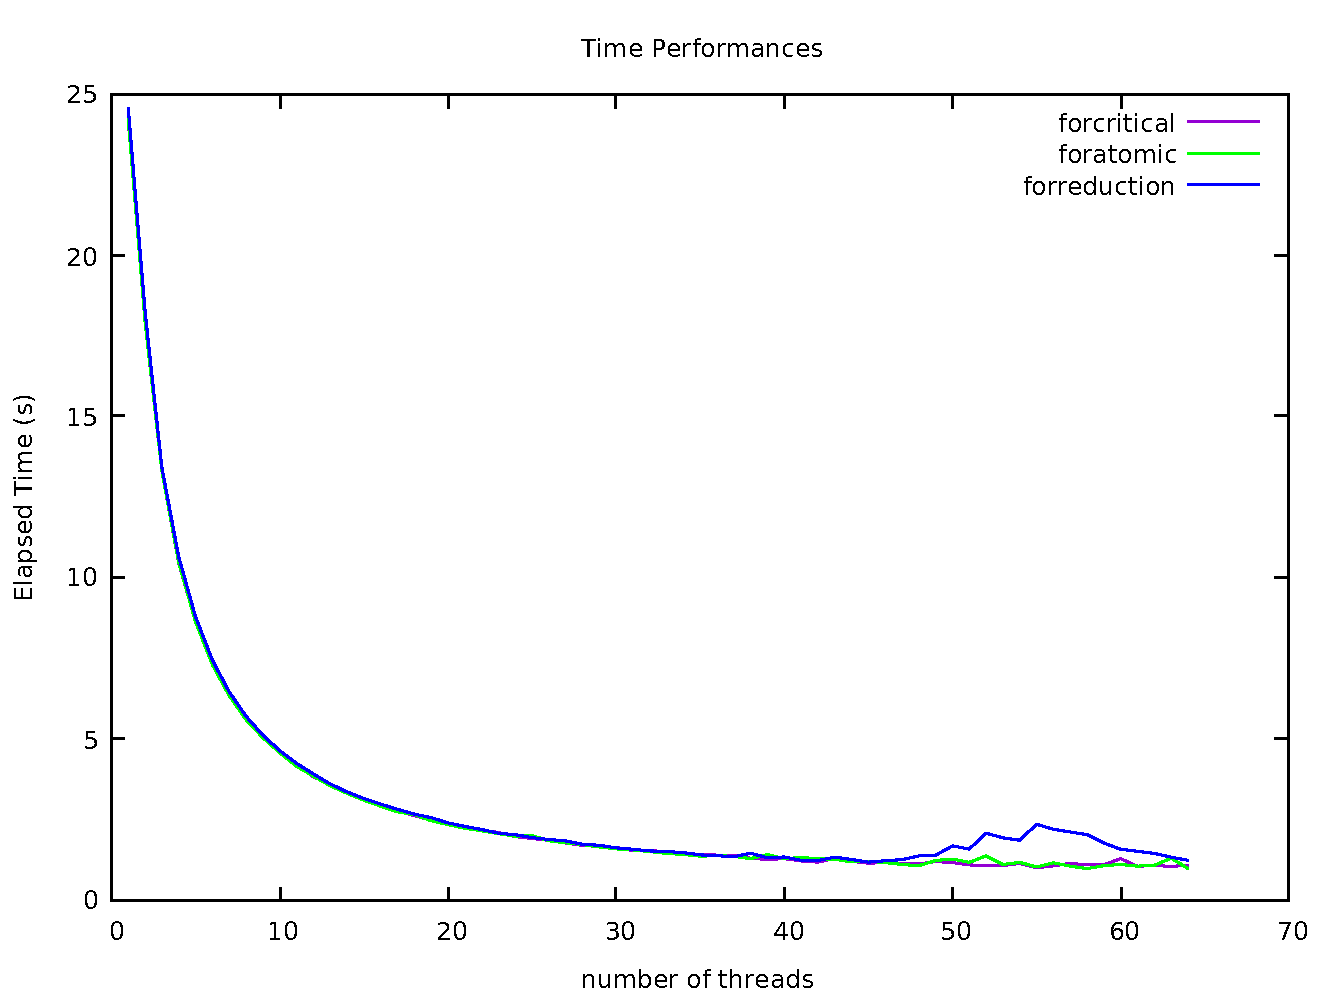
\includegraphics[width=0.75\textwidth]{../Images/Performance2.pdf}
	\label{fig:race}
	\cprotect\caption{Elapsed time as a function of the number of threads for the functions \verb+forcritical+, \verb+foratomic+ and \verb+forreduction+ (blue, with \verb+pragma for reduction+ directive).}
\end{figure}

\section{Conclusions}
\par The project aimed to calculate the value of Napier's constant $\esp$ using its definition in terms of a series:
$$\esp = \sum_{n = 0} ^{\infty} \frac{1}{n!}$$
In the project many different techniques to parallelize the computation.\\
Each technique provides great time reductions as a function of the number of the threads: the computation lasts more or less $24$ seconds when using one thread, and almost $1$ second when using $64$ threads.
In all the cases, some variations in time can be noticed when using more than $40$ threads, but the usage of the \verb+pragma critical+ and \verb+atomic+ seem to reduce this fluctuation.
\par In conclusion, with the algorithm implemented and contrary to the expectations, below $40$ threads it is quicker the implementation without the specific \verb+pragma+ directive for the \verb+for+ loop.
However, when using more than $40$ threads it is better in terms of time performances to use the \verb+pragma+ directive for the \verb+for+ loop.
It may also be safer to use the \verb+pragma critical+ and \verb+atomic+ to experience less variations in terms of computing time.

\end{document}
